\documentclass{beamer}

% \usetheme{Singapore}
% \usetheme{Malmoe}
\usetheme{Warsaw}

\usepackage[utf8]{inputenc}
\usepackage[russian]{babel}
\usepackage{cmap}
\usepackage{mathrsfs}
\usepackage{changepage}

% \useoutertheme{split}
\useoutertheme{shadow}
\usefonttheme{professionalfonts}
\usepackage{graphicx}
\usepackage{psfrag}
\beamertemplatenavigationsymbolsempty 
\DeclareMathOperator{\sign}{sign}

\setbeamertemplate{footline}[frame number]

\author{Павел Филонов \\ \href{mailto:filonovpv@gmail.com}{filonovpv@gmail.com}}
\title{Введение в машинное обучение}
\subtitle{Метрические методы классификации и регресии}

\begin{document}
\begin{frame}[plain]
    \titlepage
\end{frame}
\begin{frame}[plain]{Содержание}
  \tableofcontents
\end{frame}
\section{Гипотезы компактности и непрерывности}
\begin{frame}{Гипотезы компактности и непрерывности}

{\bf Задачи классификации и регресии:}
\begin{itemize}
    \item[] $X$ --- объекты, $Y$ --- ответы;
    \item[] $S = (x_i, y_i)_{i=1}^{\ell}$ --- обучающая выборка.
\end{itemize}

{\bf Гипотеза компактности} (для классификации):
\begin{itemize}
    \item[] {\it Близкие объекты, как правило, лежат в одном классе.}
\end{itemize}

{\bf Гипотеза непрерывности} (для регресии):
\begin{itemize}
    \item[] {\it Близким объектам соответсвуют близкие ответы.}
\end{itemize}

{\bf Формализация понятия <<близости>>:}
\begin{itemize}
    \item[] Задана функция расстояния $\rho : X \times X \rightarrow \left[ 0, \infty \right)$.
\end{itemize}

{\bf Пример.} Евклидово расстояние и его обобщение.
$$
    \rho(x_i, x_k) = \left(\sum\limits_{j=1}^{n}(x_i^j - x_k^j)^2\right)^{1/2},\;  \rho(x_i, x_k) = \left(\sum\limits_{j=1}^{n}w_j(x_i^j - x_k^j)^p\right)^{1/p}
$$
\end{frame}

\begin{frame}{Пример: рост и вес в зависимости от пола}
$N = 200$
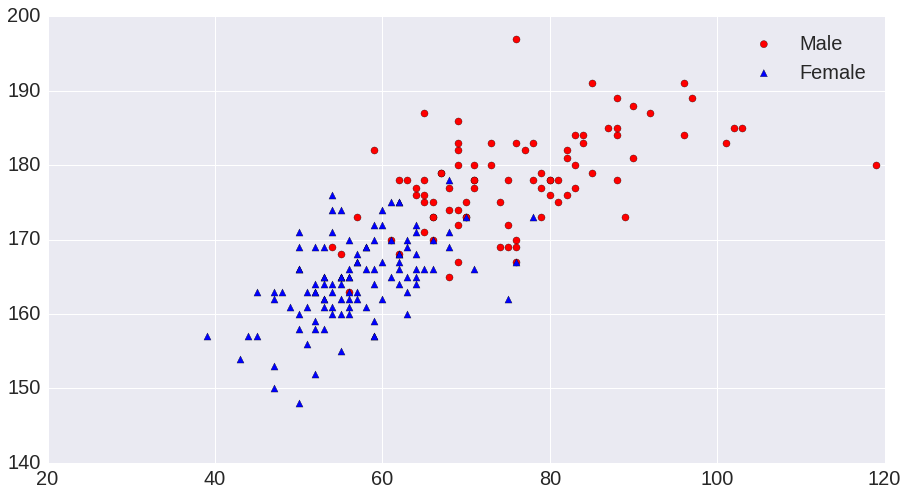
\includegraphics[width=\linewidth]{../fig/height_n_weight.png}

\footnotesize
Dataset from \url{https://vincentarelbundock.github.io/Rdatasets/datasets.html}
\end{frame}
\end{document}